\documentclass[a4paper,11pt]{article}
\usepackage[utf8]{inputenc}
\usepackage[T1]{fontenc}
\usepackage[esperanto]{babel}
\usepackage{graphicx}
\graphicspath{{./}}
\usepackage{booktabs}
\usepackage{amsmath}
\usepackage{siunitx}
\usepackage{float}
\usepackage[hidelinks]{hyperref}
\title{TP3: Modelado de la Homa Okulo}
\author{Rong ZHOU}
\newcommand{\univaddress}{3 Rue Augustin Fresnel, 57070 Metz}
\date{\today}
\newcommand{\contact}{ron@ronzz.org}

\begin{document}
\maketitle
\begin{center}
  \small Universit\'e de Lorraine, \today, \href{mailto:ron@ronzz.org}{ron@ronzz.org}, \univaddress
\end{center}

\section{Enkonduko}

La homa okulo estas verŝajne unu el la plej mirindaj konstruaĵoj de la naturo. Ekipita per lenso kapabla ŝanĝi sian fokusan distancon de ĉirkaŭ 250~mm ĝis senfinio helpe de la rektaj muskoloj, nia okulo perceptas objektojn el malproksimo same kiel el proksimo. En ĉi tiu eksperimento, ni celas rekonstrui la homan okulon per optika benko por pli bone kompreni la funkcion de la homa okulo el perspektivo de optika fiziko, precipe kiel la okulo kapablas agordi sin por fokusiĝi sur proksimajn kaj malproksimajn objektojn.

\section{Eksperimenta aranĝo}

Por ĉi tiu eksperimento, ni uzas la sekvajn ilojn:

\begin{itemize}
    \item optika benko kun gradoskalo
    \item punkta lumfonto emisianta divergajn lumradiojn
    \item travidebla kvaratita vitro servanta kiel objekto
    \item konvergaj lensoj kun nominalaj fokusaj distancoj je 10, 15 kaj 20~cm
    \item blanka ekrano
    \item diversaj teniloj por fiksi la optikan ekipaĵon al la benko
\end{itemize}

\section{Eksperimenta proceduro}

\subsection{Konfirmo de reaj fokusaj distancoj de konvergaj lensoj per autokolimacio}

Unue, ni konfirmas la fokusajn distancojn de la konvergaj lensoj, kiujn ni uzos en nia eksperimento, per la sekva aranĝo:

\begin{figure}[H]
\centering
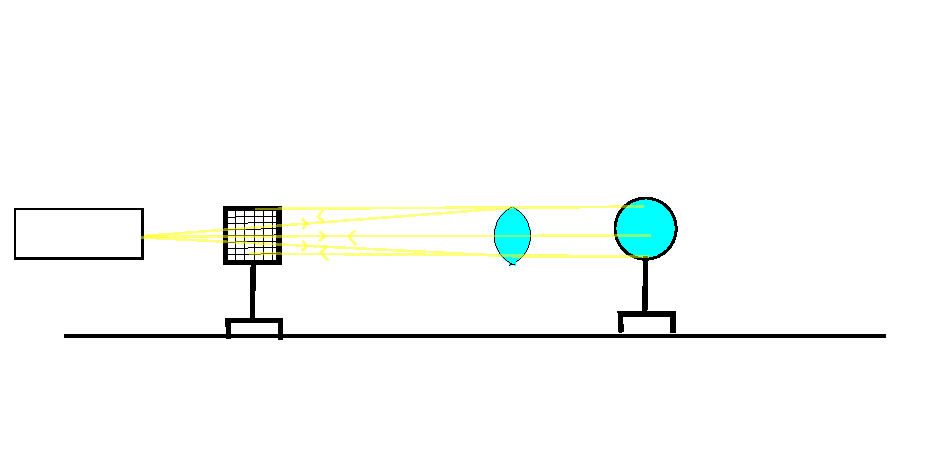
\includegraphics[width=0.9\linewidth]{autocollimation-refined.pdf}
\caption{Autokolimacia aranĝo por konfirmo de fokusaj distancoj}
\label{fig:autocollimation}
\end{figure}

Ni ricevis la sekvajn rezultojn:

\begin{table}[h]
\centering
\begin{tabular}{lrrr}
\toprule
 & \multicolumn{3}{c}{Lenso} \\
\cmidrule{2-4}
 & 1 & 2 & 3 \\
\midrule
Nominala fokusa distanco (mm) & 100 & 150 & 200 \\
Mezurita fokusa distanco (mm) & 104 & 155 & 208 \\
\bottomrule
\end{tabular}
\caption{Nominalaj kaj mezuritaj fokusaj distancoj}
\label{tab:focal-distances}
\end{table}

\subsection{Konstruado de fikcia okulo}

Ni konstruas fikcion okulon per konverga lenso, kiu reprezentas la lensan sistemon de la okulo, kaj blanka ekrano, kiu reprezentas la retinon:

\begin{figure}[H]
\centering
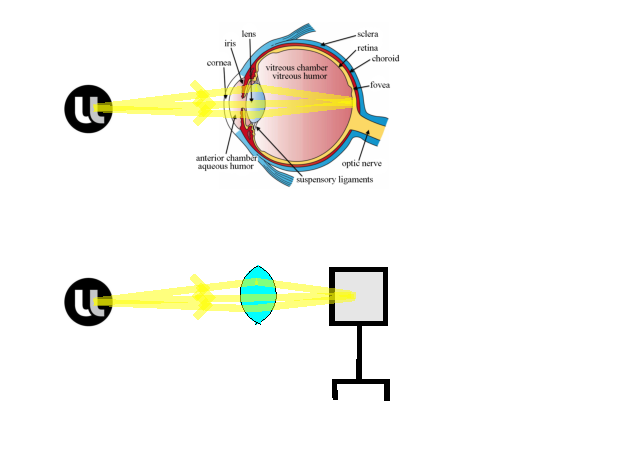
\includegraphics[width=0.9\linewidth]{eye-model.pdf}
\caption{Modelo de la fikcia okulo}
\label{fig:eye-model}
\end{figure}

\subsubsection{Fokusiĝo sur objekto en senfinio}

Ni konstruas scenaron simulantan la fokusiĝon sur objekto konsiderata infinire malproksima (lumradioj alvenantaj paralele):

\begin{figure}[H]
\centering
\includegraphics[width=0.9\linewidth]{eye-vision-infinity.pdf}
\caption{Fikcia okulo fokusita ĉe senfinio}
\label{fig:eye-infinite-focus}
\end{figure}

\subsubsection{Fokusiĝo sur proksima objekto (200 mm)}

Ni konstruas scenaron simulantan la fokusiĝon sur objekto 200~mm for de la okulo:

\begin{figure}[H]
\centering
\includegraphics[width=0.9\linewidth]{eye-vision-closeup.pdf}
\caption{Fikcia okulo fokusita sur objekto 200~mm for}
\label{fig:eye-closeup-focus}
\end{figure}

Per la leĝo de Descartes
($\frac{1}{\overrightarrow{AO}} + \frac{1}{\overrightarrow{OA'}} = \frac{1}{\overrightarrow{OF'}}$),
ni kalkulis la novan fokusan distancon bezonatan por ricevi klaran bildon sur la «retino» kiel 104~mm, kio estas eksperimente konfirmita ĉar klara bildo estas ricevata kiam ni anstataŭigas la konvergan lenso kun nominala fokusa distanco de 200~mm («okul-lenso») per konverga lenso kun nominala fokusa distanco de 100~mm.

\subsection{Eksperimentado kun lupoj por kompreni la meĥanismon de optika pligrandigo}

Post konstruo de la fikcia okulo kaj kompreno de ĝiaj optikaj meĥanismoj, ni nun provas kompreni la meĥanismojn de optika pligrandigo helpe de konvergaj lensoj (kiuj servas kiel lupoj).

La eksperimenta aranĝo estas kiel sekvas:

\begin{figure}[H]
\centering
\includegraphics[width=0.9\linewidth]{magnifying-glass.pdf}
\caption{Eksperimenta aranĝo kun lupo}
\label{fig:magnifying-glass}
\end{figure}

Do ni havas $O_{\text{okulo}}A = 600~\text{mm}$ (arbitra elekto), okulo fokusita ĉe senfinio (simulita per konverga lenso de $f_{\text{nominal}} = 200~\text{mm}$).

Per mezurilo, ni mezuris la grandecon de 11 vertikalaj kadroj de la kvaratita vitro kiel 24~mm, kio tradukiĝas al averaĝo de 2.182~mm per kadro.
Por konveno, ni izolas la kvar kadrojn super la fokusa centro, kun teoria alto de 8.727~mm kiel nia objekto ($AB = 8.727~\text{mm}$):

\begin{figure}[H]
\centering
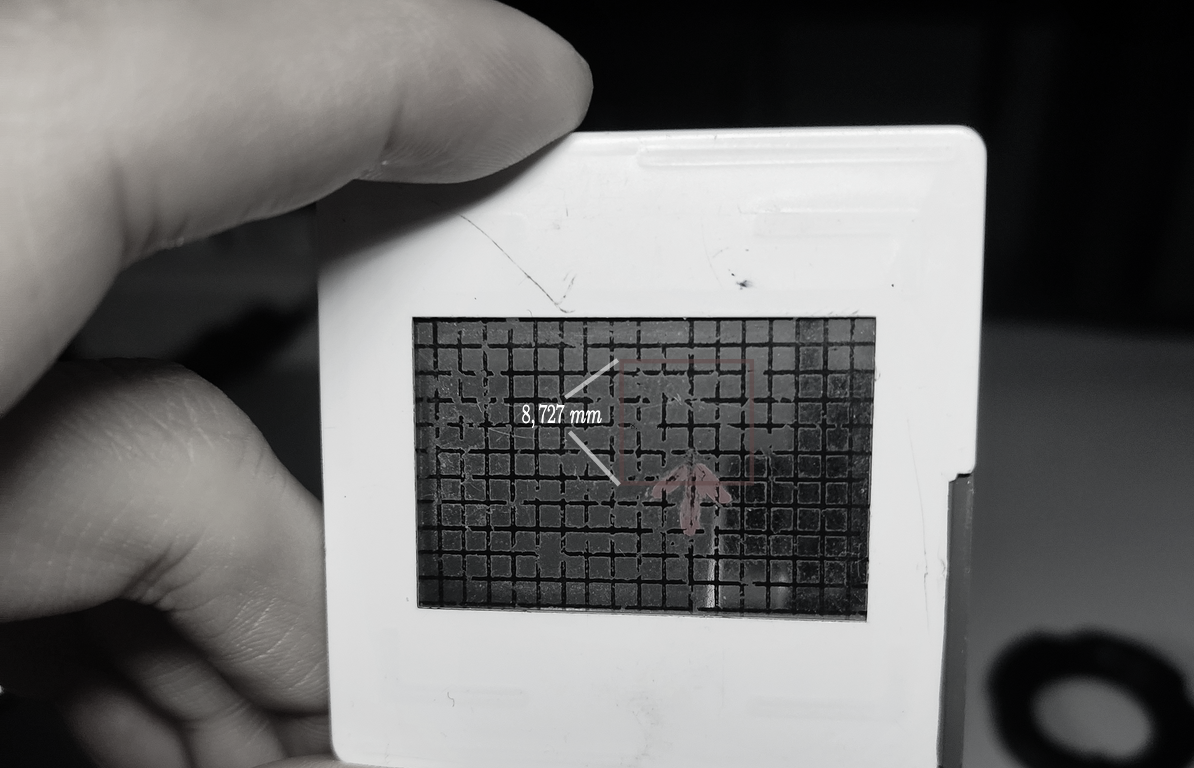
\includegraphics[width=0.9\linewidth]{grid-glass.png}
\caption{Kvaratita vitro uzata kiel objekto, kun kvar kadroj izolitaj super la fokusa centro}
\label{fig:grid-glass}
\end{figure}

Ĉi tio tradukiĝas al observoangulo $\alpha$ de ĉirkaŭ 0.0145 radianoj:

\begin{figure}[H]
\centering
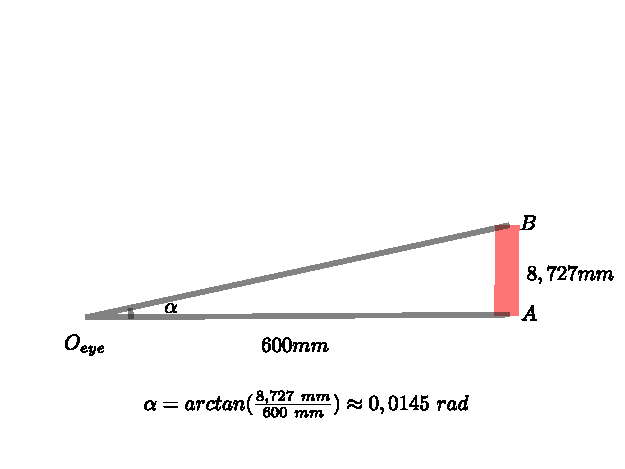
\includegraphics[width=0.9\linewidth]{observation-angle-object.pdf}
\caption{Observoangulo $\alpha$ de la objekto}
\label{fig:observation-angle-object}
\end{figure}

Por observi la pligrandigan efikon, ni metas konvergajn lensojn de diversaj fokusaj longoj inter la «okul-lenso» kaj la objekto $AB$, movante ilin ĝis klara bildo estas ricevata. Ni notas ĉi tiun pozicion kiel $O$. $AB$ estas la objekto (4 vertikalaj kadroj) kaj $A'B'$ estas la bildo projekciita sur la «retino».

Ĉar la okulo estas fokusita ĉe senfinio, la lumradioj alvenantaj al la «okul-lenso» devas esti paralelaj por formi klaran bildon sur la «retino». Tial $\alpha' = \arctan\!\left(\frac{AB}{AO}\right)$. Do la pligrandiga grandeco $M = \frac{\alpha'}{\alpha} = \frac{\arctan\!\left(\frac{AB}{AO}\right)}{0.0145~\text{rad}}$:

\begin{figure}[H]
\centering
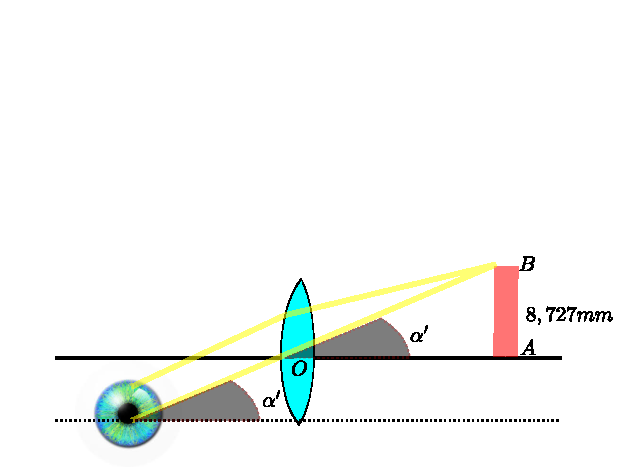
\includegraphics[width=0.9\linewidth]{magnification-magnitude.pdf}
\caption{Skemo de la pligrandiga grandeco $M$}
\label{fig:magnification-magnitude}
\end{figure}

Eksperimente ni ricevis la sekvajn mezurojn:

\begin{table}[h]
\centering
\renewcommand{\arraystretch}{1.4}
\begin{tabular}{lrrrr}
\toprule
Mezuro & \multicolumn{4}{c}{Lupo} \\
\cmidrule{2-5}
 & 1 & 2 & 3 & 4 \\
\midrule
Nominala fokusa distanco $f$ (mm) & 100 & 150 & 300 & 500 \\
$OA$ (mm) & 142 & 186 & 260 & 392 \\
$A'B'$ (mm) & 9.0 & 7.7 & 6.0 & 5.0 \\
$\frac{A'B'}{AB}$ (kalkulita) & 1.031 & 0.882 & 0.688 & 0.573 \\
$M$ (kalkulita) & 4.22 & 3.22 & 2.31 & 1.53 \\
$\frac{M}{\frac{A'B'}{AB}}$ & 4.092 & 3.654 & 3.356 & 2.671 \\
\bottomrule
\end{tabular}
\caption{Eksperimentaj pligrandigaj mezuroj}
\label{tab:magnification}
\end{table}

El ĉi tio ni povas atesti, ke la homa okula lenso «malgrandigas» bildojn antaŭ ol transdoni ilin al la retino. Ĉar ni rimarkis, ke la vidkampo (reprezentita per la nombro de videblaj kadroj sur la ekrano) estas ĉiam pli limigita kun pli altaj pligrandigaj grandecoj, ni konkludas, ke ĉi tio estas celkonforma por konservi la vidkampon dum ni rigardas objektojn multe pli grandajn ol nia okulo!

Krome, grafike prezentante $M$ kontraŭ $\frac{1}{f}$:

\begin{figure}[H]
\centering
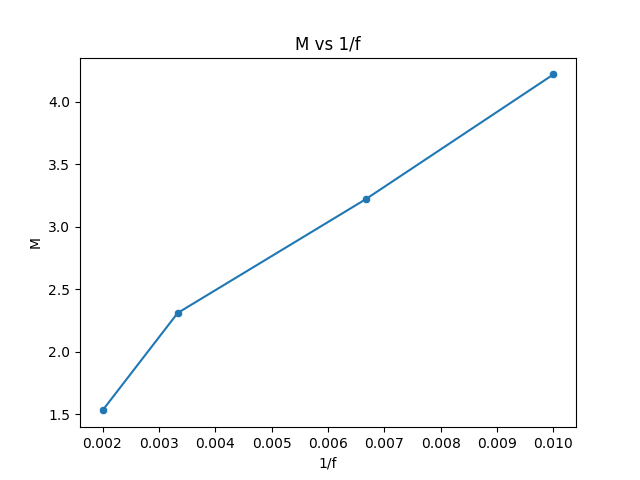
\includegraphics[width=0.9\linewidth]{M-f.png}
\caption{Grafeo de $M$ kontraŭ $\frac{1}{f}$}
\label{fig:M-f}
\end{figure}

Ni observas preskaŭ linearan rilaton inter la du, kiel atendite.

\section{Konkludo}

En ĉi tiu eksperimento, ni rekonstruis homan okulon per optikaj geometriaj analogaĵoj por kompreni kiel homa okulo kapablas fokusiĝi sur objektojn de malsamaj distancoj. Ni poste metis konvergajn lensojn de diversaj fokusaj longoj antaŭ nia fizika analogiga okulo por kompreni la funkcion de lupoj. Niaj eksperimentaj rezultoj konkordas kun teoriaj derivaĵoj.

\section{Bibliografio}

\begin{thebibliography}{99}
\end{thebibliography}

\section{Aldonaĵo}

Python-kodo uzita por grafiki $M$ kontraŭ $\frac{1}{f}$:

\begin{verbatim}
import seaborn as sns
import matplotlib.pyplot as plt
import pandas as pd

# Your data (converted to proper floats)
data = pd.DataFrame({
    "inv_f": [0.01, 0.00666666666666667, 0.00333333333333333, 0.002],
    "M": [4.22, 3.22, 2.31, 1.53]
})

# Plot
sns.scatterplot(data=data, x="inv_f", y="M")

# Optional: add line
sns.lineplot(data=data, x="inv_f", y="M")

plt.xlabel("1/f")
plt.ylabel("M")
plt.title("M vs 1/f")
plt.show()
\end{verbatim}

\end{document}
